\documentclass{standalone}

\usepackage{tikz}
\usepackage[T1]{fontenc}
\usepackage[tt=false, type1=true]{libertine}
\usepackage[varqu]{zi4}
\usepackage[libertine]{newtxmath}
\usepackage{calc}
\usepackage{calc}

\newcommand{\SqueezeMidOp}[3]{#1 \!#2\! #3}

\usetikzlibrary{shapes, positioning, calc}

\begin{document}

{\scriptsize
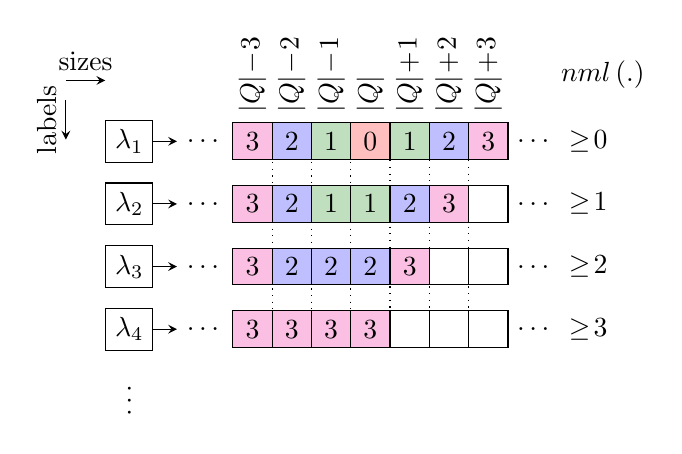
\begin{tikzpicture}
  \newcommand\maxsizediff{3}
  \newcommand\listnum{4}

  \newcommand\listentrynum{\the\numexpr\maxsizediff * 2 + 1}
  \newcommand\midrow{\the\numexpr\maxsizediff + 1}

  \newcommand\arraypartspacing{0.015} % 0.03 for thick
  \newcommand\listpartspacing{0.3}
  \newcommand\listspacing{0.25}
  \newcommand\listdir{right}
  \newcommand\lbldir{below}
  \newcommand\sizedir{above}

  \tikzset{ptr/.style={->, >=stealth}}

  \tikzset{ilentry/.style={draw, minimum height=0.4675cm, minimum width=0.5cm}}
  \tikzset{processedilentry/.style={ilentry, fill opacity=0.25, text opacity=1}}
  \tikzset{ilentrylb/.style={minimum height=0.4675cm, minimum width=0.5cm}}

  \tikzset{ilentrylb0width/.style={minimum width=0.5cm}}
  \tikzset{ilentrylb0/.style={processedilentry, fill=red}} %, ilentrylb0width}}

  \tikzset{ilentrylb1/.style={processedilentry, fill=black!50!green}}
  \tikzset{ilentrylb11width/.style={minimum width=0.35cm}}
  \tikzset{ilentrylb12width/.style={minimum width=0.65cm}}
  \tikzset{ilentrylb11/.style={ilentrylb1}} %, ilentrylb11width}}
  \tikzset{ilentrylb12/.style={ilentrylb1}} %, ilentrylb12width}}

  \tikzset{ilentrylb2/.style={processedilentry, fill=blue}}
  \tikzset{ilentrylb21width/.style={minimum width=0.75cm}}
  \tikzset{ilentrylb22width/.style={minimum width=0.8cm}}
  \tikzset{ilentrylb21/.style={ilentrylb2}} %, ilentrylb21width}}
  \tikzset{ilentrylb22/.style={ilentrylb2}} %, ilentrylb22width}}

  \tikzset{ilentrylb3/.style={processedilentry, fill=magenta}}
  \tikzset{ilentrylb31width/.style={minimum width=0.5cm}}
  \tikzset{ilentrylb32width/.style={minimum width=1cm}}
  \tikzset{ilentrylb31/.style={ilentrylb3}} %, ilentrylb31width}}
  \tikzset{ilentrylb32/.style={ilentrylb3}} %, ilentrylb32width}}

  \node[ilentry] at (0, 0) (il1) {$\lambda_1$};
  \node[\listdir=\listpartspacing of il1] (il1-0) {\ldots};
  \draw[ptr] (il1) -- (il1-0);

  \foreach \size/\lb/\lbstyle [count=\previndex from 0] in {1/3/31, 2/2/21, 3/1/11, 4/0/0, 5/1/12, 6/2/22, 7/3/32, 8/\ldots/}{
    \node[\listdir=-\arraypartspacing of il1-\previndex, ilentrylb\lbstyle] (il1-\size) {\lb};
  }

  \foreach \labelid [count=\prevlabelid from 1] in {2, ..., \listnum}{
    % label
    \node[\lbldir=\listspacing of il\prevlabelid, ilentry] (il\labelid) {$\lambda_\labelid$};
    % first list entry
    \node[\listdir=\listpartspacing of il\labelid] (il\labelid-0) {\ldots};
    \draw[ptr] (il\labelid) -- (il\labelid-0);
  }

  \foreach \size/\lb/\lbcolor/\lbwidth [count=\previndex from 0] in {1/3/ilentrylb3/ilentrylb31width, 2/2/ilentrylb2/ilentrylb21width, 3/1/ilentrylb1/ilentrylb11width, 4/1/ilentrylb1/ilentrylb0width, 5/2/ilentrylb2/ilentrylb12width, 6/3/ilentrylb3/ilentrylb22width, 7//ilentry/ilentrylb32width, 8/\ldots//}{
    % add \lbwidth for unequally-sized partitions
    \node[\listdir=-\arraypartspacing of il2-\previndex, \lbcolor] (il2-\size) {\lb};
  }

  \foreach \size/\lb/\lbcolor/\lbwidth [count=\previndex from 0] in {1/3/ilentrylb3/ilentrylb31width, 2/2/ilentrylb2/ilentrylb21width, 3/2/ilentrylb2/ilentrylb11width, 4/2/ilentrylb2/ilentrylb0width, 5/3/ilentrylb3/ilentrylb12width, 6//ilentry/ilentrylb22width, 7//ilentry/ilentrylb32width, 8/\ldots//}{
    % add \lbwidth for unequally-sized partitions
    \node[\listdir=-\arraypartspacing of il3-\previndex, \lbcolor] (il3-\size) {\lb};
  }

  \foreach \size/\lb/\lbcolor/\lbwidth [count=\previndex from 0] in {1/3/ilentrylb3/ilentrylb31width, 2/3/ilentrylb3/ilentrylb21width, 3/3/ilentrylb3/ilentrylb11width, 4/3/ilentrylb3/ilentrylb0width, 5//ilentry/ilentrylb12width, 6//ilentry/ilentrylb22width, 7//ilentry/ilentrylb32width, 8/\ldots//}{
    % add \lbwidth for unequally-sized partitions
    \node[\listdir=-\arraypartspacing of il4-\previndex, \lbcolor] (il4-\size) {\lb};
  }

  \foreach \sign/\start/\interval in {-/1/{\maxsizediff, ..., 1}, +/\the\numexpr\midrow+1/{1, ..., \maxsizediff}}{
    \foreach \sizediff [count=\index from \start] in \interval{
      \node[\sizedir=0 of il1-\index] (il-sizediff-\index) {\rotatebox{90}{$\SqueezeMidOp{|Q|}{\sign}{\sizediff}$}};
    }
  }
  \node[\sizedir=0 of il1-\midrow] (il-sizediff-\midrow) {\rotatebox{90}{$|Q|$}};
  \node[\lbldir=0.25 of il\listnum] {\rotatebox{90}{\ldots}};

  \draw[ptr] ($(il1.north west)+(-0.5,0.25)$) -- node[left] {\rotatebox{90}{labels}} ++(0,-0.5);
  \draw[ptr] ($(il1.north west)+(-0.5,0.5)$) -- node[above] { sizes} ++(0.5, 0);

  \foreach \lb in {1, ..., \the\numexpr\maxsizediff}{
    \newcommand\posa{\the\numexpr\midrow-\lb}
    \newcommand\posb{\the\numexpr\midrow+\lb}

    \draw[dotted] ($(il1-\posa.north east)-(\arraypartspacing/2, 0)$) -- ($(il\listnum-\posa.north east)-(\arraypartspacing/2, 0)$);
    \draw[dotted] ($(il1-\posb.south west)+(\arraypartspacing/2, 0)$) -- ($(il\listnum-\posb.north west)+(\arraypartspacing/2, 0)$);
  }

  \node[\listdir=2*\listspacing of il-sizediff-7] (nml) {$nml\left( . \right)$};
  \foreach \listid [count=\nml from 0] in {1, ..., 4}{
    \node[\listdir=0 of il\listid-8] (il\listid-nml) {$\SqueezeMidOp{}{\geq}{\nml}$};
  }
\end{tikzpicture}}

\end{document}
